\documentclass[tikz,border=8pt]{standalone}
\usepackage{amsmath}
\usetikzlibrary{arrows.meta,calc,angles,quotes}
\definecolor{ink}{HTML}{17324D}
\definecolor{accent}{HTML}{0F766E}
\definecolor{gold}{HTML}{C28524}
\begin{document}
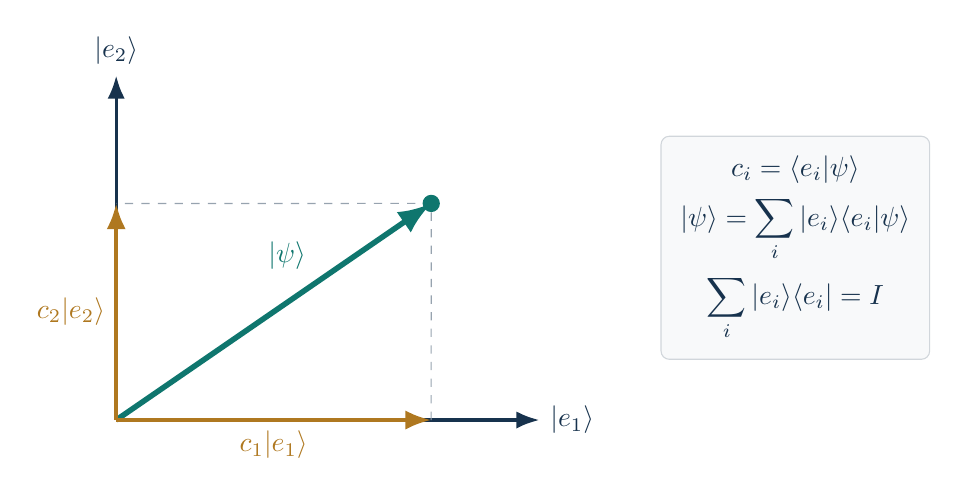
\begin{tikzpicture}[>=Latex,font=\sffamily,scale=1.25]
 \coordinate (O) at (0,0);
 \coordinate (Eone) at (4.3,0);
 \coordinate (Etwo) at (0,3.5);
 \coordinate (Psi) at (3.2,2.2);
 \draw[->,ink,line width=1.2pt] (O)--(Eone) node[right] {$|e_1\rangle$};
 \draw[->,ink,line width=1.2pt] (O)--(Etwo) node[above] {$|e_2\rangle$};
 \draw[dashed,ink!45] (3.2,0)--(Psi)--(0,2.2);
 \draw[->,accent,line width=2pt] (O)--(Psi)
   node[pos=.64,above left] {$|\psi\rangle$};
 \draw[->,gold!90!black,line width=1.4pt] (O)--(3.2,0)
   node[midway,below] {$c_1|e_1\rangle$};
 \draw[->,gold!90!black,line width=1.4pt] (0,0)--(0,2.2)
   node[midway,left] {$c_2|e_2\rangle$};
 \fill[accent] (Psi) circle (2.5pt);
 \node[align=center,ink,draw=ink!20,rounded corners=3pt,fill=ink!3,
       inner sep=7pt] at (6.9,1.75)
 {$c_i=\langle e_i|\psi\rangle$\\[4pt]
  $\displaystyle |\psi\rangle=\sum_i|e_i\rangle\langle e_i|\psi\rangle$\\[4pt]
  $\displaystyle \sum_i|e_i\rangle\langle e_i|=I$};
\end{tikzpicture}
\end{document}
